\chapter{\textit{Clean Pool Robot}}
Consta, neste capítulo, uma visão geral sobre o produto final, o
\textit{Clean Pool Robot}. Em seguida apresenta-se as especificações técnicas
do robô, bem como as suas restrições. Depois detalha-se os sistemas que compõem
o \textit{Clean Pool Robot}.

\section{Visão Geral}
O \textit{Clean Pool Robot} é um equipamento robótico que visa auxiliar a limpeza de
piscinas. O mecanismo de limpeza do robô é composto por dois métodos, o
primeiro baseia-se em esfregar o chão para desprender as sujeiras do piso da
piscina e o segundo a sucção das mesmas.

O primeiro método tem foco nos rolos de limpeza que estão situados na parte
inferior frontal e traseira do robô. Os rolos de limpeza realizam movimentos
giratórios fazendo com que suas cerdas entrem em contato com o chão retirando
impurezas. Após esfregar, é realizado a sucção das impurezas desprendidas do
piso da piscina, bem como outras impurezas que estiverem próximas à área de
atuação do robô. Por meio de uma bomba, a água é sugada por uma abertura
situada na parte inferior e passa por um filtro. As impurezas ficam retidas
no sistema de filtragem. Os filtros da piscina devem ser trocados periodicamente
para garantir o funcionamento ideal do \textit{Clean Pool Robot}. O sistema de expulsão
de água será responsável por direcionar o jato de água da saída da bomba de
forma a auxiliar na movimentação do robô.

O \textit{Clean Pool Robot} é de fácil manuseio pelo usuário. Inicialmente deve-se
esticar o fio de alimentação do robô e inseri-lo de forma inclinada na
superfície da piscina para auxiliar no processo de descida do robô. Recomenda-se
também que o robô seja lançado na piscina no meio da largura maior, evitando
que o fio fique totalmente esticado quando o robô estiver na quina oposta do
lançamento. É estritamente proibido o funcionamento do robô junto a pessoas
dentro da piscina. Quando o CPR estiver no fundo da piscina, ligar o fio externo
na tomada e aguardar a completa limpeza da piscina. Ao final do processo,  o
usuário deve desligar o CPR da tomada e retirar o robô da piscina, puxando pelo
cabo. Limpar os filtros do robô e guardar fora d'água para a próxima limpeza.
Caso o usuário não esteja satisfeito com o nível de limpeza, é sugerido a
repetição do mesmo processo.

\subsection{Restrições}
O produto desenvolvido é responsável apenas pela retirada da sujeira decantada
no fundo da piscina. Além disso, o \textit{Clean Pool Robot}, primeira
versão, possui as seguintes restrições quanto ao tipo de piscina:

\begin{itemize}
\item Formato retangular;
\item A junção entre as paredes e o fundo da piscina devem formar um ângulo de 90 graus;
\item Superfície sem inclinações ou degraus;
\item Profundidade máxima de dois metros;
\item Área máxima de 25 x 20 metros (piscinas semiolímpicas).
\end{itemize}

\subsection{Especificações Técnicas}

\begin{table}[h]
\centering
\caption{Especificações Técnicas}
\label{spec-tec}
\begin{tabular}{@{}cccc@{}}
\toprule
\multicolumn{2}{c}{\textbf{Dimensões}}                                                                                                                                       & \multicolumn{2}{c}{490 mm x 300 mm}                                                                                                                                           \\
\multicolumn{2}{c}{\textbf{Material}}                                                                                                                                        & \multicolumn{2}{c}{Polipropileno e Aço}                                                                                                                                       \\
\multicolumn{2}{c}{\textbf{Velocidade do Robô}}                                                                                                                              & \multicolumn{2}{c}{0,15 m/s - 0,38 m/s}                                                                                                                                       \\ \midrule
\multicolumn{4}{c}{}                                                                                                                                                                                                                                                                                                                                         \\
\textbf{Sensor de Distância}   & HC-SR04                                                                                                                                     & \textbf{Rodas}          & Plástico - 360º                                                                                                                                     \\
\textbf{Servo - Rodas}         & Micro servo 9g SG90 Tower Pro                                                                                                               & \textbf{Fonte Chaveada} & 220 Vca - 12 Vca                                                                                                                                    \\
\textbf{Servo - Bomba}         & SM-S4306R                                                                                                                                   & \textbf{Filtros}        & Poly Flow                                                                                                                                           \\ \midrule
\textbf{Rolo de Limpeza}       & \begin{tabular}[c]{@{}c@{}}Material : Vinil\\ Dimensões: comprimento-300mm\\ diâmetro out-60mm\\ diâmetro in-30mm\\ massa-450g\end{tabular} & \textbf{Bomba}          & \begin{tabular}[c]{@{}c@{}}BILGE - 1800 GPH\\ Peso: 3 kg\\ Tensão: 12 V DC\\ Corrente: 3,3 A\\ Formato: Cilíndrico\\ Operação:até 3,7m\end{tabular} \\
\multicolumn{2}{c}{\textbf{Motores - Escovas}}                                                                                                                               & \multicolumn{2}{c}{AK080/16.5ML12S6800S}                                                                                                                                      \\ \midrule
\textit{\textbf{Raspberry Pi}} & \textit{Raspberry Pi 2}                                                                                                                     & \textbf{Arduino}        & Arduino Uno                                                                                                                                         \\ \bottomrule
\end{tabular}
\end{table}

\section{Sistemas}
\subsection{Sistemas Estruturais}
A parte estrutural do projeto foi divida nas seguintes áreas: \textit{design},
sistema de alimentação elétrico, sistema de locomoção, sistema de limpeza e
sistema de vedação. Cada uma dessas áreas são descritas a seguir.

\subsubsection{\textit{Design}}
O \textit{design} do CPR sofreu várias alterações ao longo da execução do
projeto. Inicialmente o projeto foi idealizado e projetado em um \textit{sketch}
a mão livre, onde apresentava um duto superior estilo chaminé com quatro saídas,
além de escovas nas partes internas da estrutura. A figura abaixo apresenta o
primeiro modelo de robô idealizado. Após conversas entre a equipe e os professores,
o projeto foi alterado para uma estrutura com escovas localizadas mais nas
laterais do robô, para minimizar o efeito do choque da estrutura com as paredes
da piscina. Também sofreu alteração o \textit{design} do duto superior, que
passou a ter um formato curvo e único de saída do jato d’água. As Figuras
\ref{fig:croqui-v1} e \ref{fig:croqui-v2} mostram o CPR em seu primeiro
croqui e uma outra versão, projetada no \textit{software} \textsf{CATIA}.
\begin{figure}[h]
  \centering
  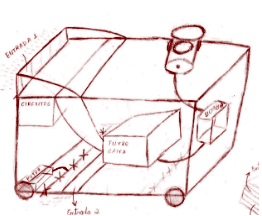
\includegraphics[width=0.4\textwidth]{figuras/croqui-v1.png}
  \caption{Primeiro croqui do \textit{Clean Pool Robot}(\textsf{Autoria do Autor}).}
  \label{fig:croqui-v1}
\end{figure}
\FloatBarrier

\begin{figure}[h]
  \centering
  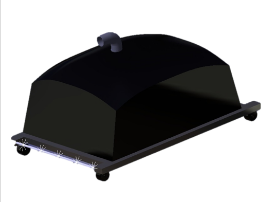
\includegraphics[width=0.4\textwidth]{figuras/croqui-v2.png}
  \caption{\textit{Design}, projetado no \textsf{CATIA}, do \textit{Clean Pool Robot}(\textsf{Autoria do Autor}).}
  \label{fig:croqui-v2}
\end{figure}
\FloatBarrier

Por motivo de resistência ao movimento o formato do robô foi modificado para
melhor aproveitamento das forças hidrodinâmica envolvidas, as alterações no
desenho inicial foram feitas com a intenção de diminuir a força de arrasto, a
estrutura conta agora com cantos e arestas arredondadas conforme as
Figuras \ref{fig:croqui-v1} e \ref{fig:croqui-v2}.

Na fase de montagem e integração dos sistemas que compõem o robô, percebeu-se
que o \textit{design} programado era inviável de ser produzido com os recursos
desse projeto. Dessa forma, houve alterações nesta estrutura, a fim de viabilizar
a montagem e funcionamento. Assim, a versão 3 do \textit{design} do robô é
apresentada an Figura \ref{fig:cpr-v3}, onde a superfície externa é retangular, com base do mesmo
tamanho da estrutura e com as rodas posicionadas na parte interna, sem pontas
sobressaltadas como no modelo anterior.

\begin{figure}[h]
  \centering
  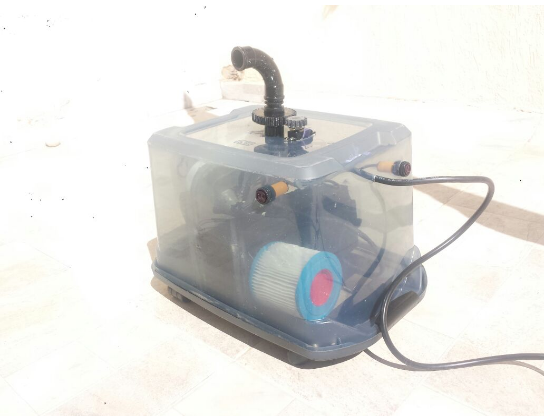
\includegraphics[width=0.6\textwidth]{figuras/cpr-v3.png}
  \caption{\textit{Design}, versão 3, do \textit{Clean Pool Robot}(\textsf{Autoria do Autor}).}
  \label{fig:cpr-v3}
\end{figure}
\FloatBarrier

\subsubsection{Sistema de Alimentação Elétrica}
O sistema de alimentação elétrica é o ponto de convergência de todos os circuitos,
pois a partir dele todos os equipamentos descritos nos demais sistemas poderão
realizar suas funcionalidades. Esse sistema é composto por uma alimentação
externa, ligada a uma fonte chaveada que, por sua vez, fará a alimentação na
tensão correta de cada equipamento.

A alimentação externa do \textit{Clean Pool Robot} é feita por meio de um cabo
de energia dimensionado de forma a suprir a potência elétrica dos equipamentos
embarcados no sistema, além de garantir que o robô percorra, sem limitação de
distância, toda a extensão da piscina. O CPR será alimentado por uma tomada
com tensão de 220 V (padrão Brasília), entretanto, os equipamentos internos são
alimentados em diferentes tensões, fazendo com que seja necessário o uso de uma
fonte chaveada para a redução da tensão de alimentação de cada equipamento.

Para o dimensionamento do comprimento do cabo foi calculado uma distância média
da tomada até a borda da piscina, somado ao maior comprimento possível para
deslocamento do robô, assim o cabo terá idealmente 30 m. No entanto, na execução
do protótipo, devido ao  limitado recurso financeiro, foram utilizados 4 m de
cabo, o suficiente para execução dos testes e prova de conceito com o protótipo,
quando usado com uma extensão. 

A bitola do cabo de energia foi dimensionada de acordo com a potência consumida
pelo CPR. Para o robô de piscina deste projeto, a potência total máxima
fornecida ao robô é de 120 W, e a corrente máxima que é fornecida pela fonte
ao fio é de 10 A, em corrente contínua. Assim, utilizando a tabela abaixo temos
que a bitola ideal para o fio é de 2,5 mm\textsuperscript{2}, para o sistema
\textsf{CC}, desde que tenha no máximo 5 m de comprimento.

\begin{figure}[h]
  \centering
  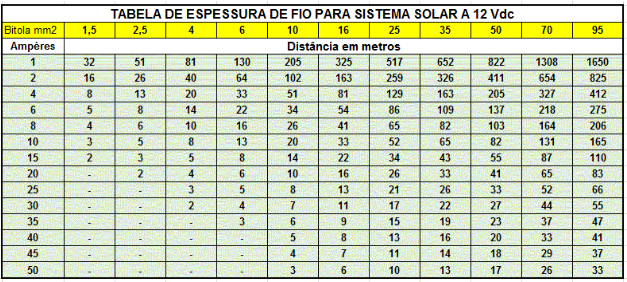
\includegraphics[width=\textwidth]{figuras/espessura-fio-cc.png}
  \caption{Espessura de fio para sistemas em corrente contínua.}
  \label{fig:espessura-fio-cc}
\end{figure}
\FloatBarrier

Para alimentação interna do robô, que deve ser feita em duas tensões diferentes,
foi escolhido o uso de uma fonte chaveada (\textit{switched-mode power supply})
devido as características de baixo volume, peso e maior eficiência em comparação
às fontes de alimentação convencionais. Os parâmetros elétricos da fonte escolhida
são: 110/220 Volts AC para 12 Volts e 10 Ampéres DC.

\begin{figure}[h]
  \centering
  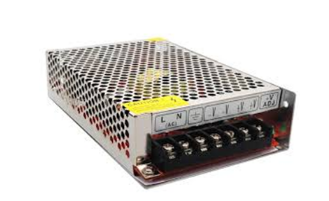
\includegraphics[width=0.6\textwidth]{figuras/power-supply.png}
  \caption{Fonte de alimentação chaveada.}
  \label{fig:power-supply}
\end{figure}
\FloatBarrier

Como o equipamento elétrico estará funcionando em meio aquoso, é necessário
o uso de  elementos de proteção. No CPR foi acoplado um disjuntor e um
regulador de tensão. O disjuntor utilizado é um termomagnético com corrente
máxima de 15 A. O mesmo foi escolhido com a finalidade somente de proteção
do circuito, já que o equipamento não deve ser acionado na piscina ao
mesmo tempo em que o usuário estiver na piscina. 

\subsubsection{Sistema de Locomoção}
O sistema de locomoção do CPR é formado pelo conjunto das rodas, duto de
propulsão, bomba e motores. A bomba e o motor são equipamentos comuns também
aos  sistemas de limpeza e automação, respectivamente. Entretanto, serão
apresentados no sistema de limpeza, ainda que sejam parte integrante dos demais.

Para a locomoção do equipamento, o robô contará com um conjunto de quatro
rodas com liberdade de 360 graus, localizadas nas extremidades do aparelho,
além de duas rodas na parte central do CPR. O primeiro modelo de rodas
escolhidas para o robô eram de metal, pela facilidade de oxidação das mesmas,
elas foram substituídas por rodas de plástico. As quatro primeiras rodas de
locomoção que se encontram nas extremidades do CPR são apresentadas na
Figura \ref{fig:wheel-base}. Essas rodas direcionam o seu movimento de acordo
com a direção do jato de água, oriundo do bocal. Já as duas rodas centrais
possuem a função de direcionar o movimento do robô, de forma a percorrer
um caminho orientado.

\begin{figure}[h]
  \centering
	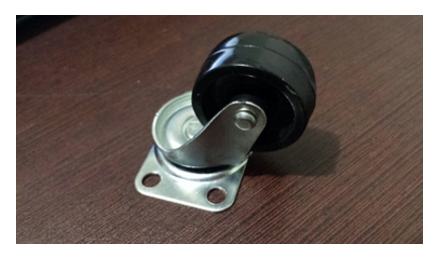
\includegraphics[height=5cm]{figuras/wheel-market.png}
	\quad
	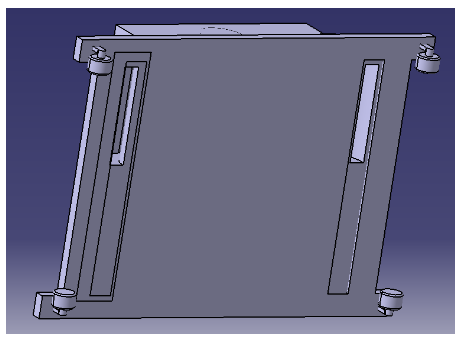
\includegraphics[height=5cm]{figuras/catia-base.png}
  \caption{Rodas utilizadas para a locomoção do robô e posicionamento na base da estrutura - modelo 01}
  \label{fig:wheel-base}
\end{figure}
\FloatBarrier

A Figura \ref{fig:wheels} mostra os modelos de rodas utilizadas, além da
sua fixação na base do robô, após a troca das rodas de metal por rodas
de plástico.

\begin{figure}[h]
  \centering
	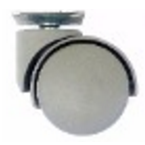
\includegraphics[height=5cm]{figuras/plastic-wheel.png}
	\quad
	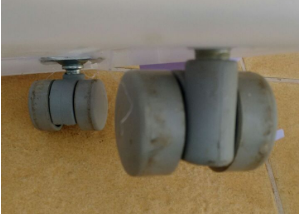
\includegraphics[height=5cm]{figuras/plastic-wheels-base.png}
  \caption{Rodas de plástico finais do robô.}
  \label{fig:plastic-wheel-base}
\end{figure}
\FloatBarrier

A água que é ejetada do sistema de filtragem é devolvida para a piscina, auxiliando
assim a limpeza geral de todo o volume em que o robô esta submerso. A água filtrada
é direcionada para uma saída que se localiza na parte superior do produto. O duto
de saída é um bocal direcionável localizado na parte superior do robô responsável
por sua locomoção. Esse bocal se move nas 4 direções principais, isto é, nos ângulos
de 0, 90, 180 e 270 graus, proporcionando ao robô a locomoção necessária para o
cumprimento da rota de limpeza.

O duto de propulsão tem o diâmetro de 1” (25,4mm) e foi construído de forma que a
água mude de direção sem que haja vazamentos e que o servo responsável pela rotação
não entre em contato com a água. Para isso, foi utilizado um servo motor e duas
engrenagens, como ilustrado na imagem abaixo. O controle do duto ocorre por meio
de um algoritmo que verifica constantemente o sinal identificado pelo sensor de
distância enquanto o robô está se movimentando. Ao identificar uma parede, é
desligado a bomba e aciona-se o servo motor resultando no giro das engrenagens e,
consequentemente,  no giro do duto. Após o término desse giro, a bomba novamente
é acionada, possibilitando o movimento com a nova orientação do jato d’água.

\begin{figure}[h]
  \centering
  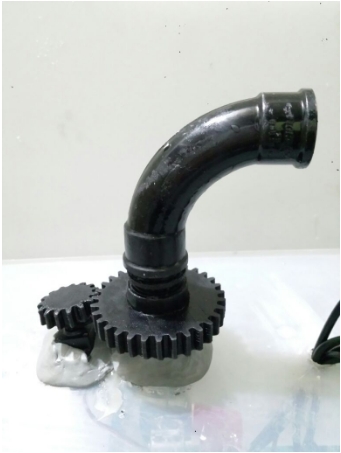
\includegraphics[width=0.4\textwidth]{figuras/duct-real.png}
  \caption{Duto de propulsão do CPR.}
  \label{fig:duct-real}
\end{figure}
\FloatBarrier

\subsubsection{Sistema de Limpeza}
O sistema de limpeza é responsável por operações de filtragem e escovação de detritos, dessa forma os seguintes componentes compõem esse sistema: filtros, rolos de limpeza, motores e bomba. A partir das definições iniciais do projeto fez se necessário considerar o dimensionamento e os materiais necessários para construção desse sistema. 

   Para filtragem foi definido o uso de  dois tipos de filtros: um de maior tamanho, denominado filtro secundário, que tem a função de realizar uma pré-filtragem retendo folhas, plásticos, cabelos, e outros objetos de maior tamanho, e outro filtro denominado filtro principal, que é responsável por retirar as impurezas menores da água. O filtro principal será um elemento filtrante na forma cilíndrica comumente utilizado na filtragem de caixas d’águas, com temperatura de operação de  5 ºC – 50 ºC, vazão de 2.200 litros/hora, e com um grau de filtração de 50 micra (um grão de areia tem entre 200 a 500 micra).

A partir das especificações definidas no design do CPR, os rolos de limpeza estão localizados na parte frontal e traseira do robô, e tem duas funções: a principal que é auxiliar na remoção das impurezas do fundo da piscina, e a função secundária que é auxiliar na sustentação do robô.
 Para o processo principal, a remoção das pequenas partículas depositadas no fundo da piscina, o rolo irá deslizar sob a superfície, sem que seja produzido muito atrito, para que não altere a velocidade total do robô e não danifique a superfície. As especificações para construção dos rolos de limpeza foram definidas em função da estrutura do robô. Com as alterações na estrutura do robô, foram feitas adaptações nas escovas.

Definiu-se primeiramente utilizar rolos de limpeza de formato cilíndrico e de \textsf{Nylon}, afim de que a medida que as rodas do robô se movam, os rolos também possam acompanhar o movimento sem maiores problemas. Porém, a dificuldade em encontrar fabricantes e modelos em Brasília e devido também ao elevado custo decidiu-se pela fabricação dos rolos de limpeza. Para a fabricação usou-se um tubo 50 mm de PVC e um revestimento de polímero, a fibra de vinil.  A utilização de um polímero possui várias vantagens, tais como: baixa densidade, alta resistência à corrosão, baixo custo de aquisição, coeficiente de atrito baixo e grande flexibilidade. O baixo custo e densidade foram os principais motivos para a realização desse ajuste.

\begin{figure}[h]
  \centering
  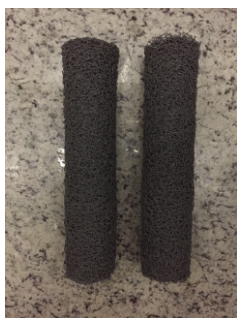
\includegraphics[width=0.6\textwidth]{figuras/rolo-fim.png}
  \caption{Rolo de fibra de vinil.}
  \label{fig:rolo-fim}
\end{figure}
\FloatBarrier

Para rotacionar os rolos de limpeza foram planejados utilizar dois motores elétricos. Para isso, a transmissão do torque se dará por engrenagens. Para a escolha dos motores foram utilizados 2 critérios: rotação dos rolos de limpeza e a massa das mesmas. O motor deverá ser capaz de rotacionar o eixo dos rolos entre 2000 e 3000 RPM e, considerando que elas têm massa igual a 250 g, ter torque suficiente para realizar o giro. A partir desses requisitos foi definido  o modelo de motor a ser usado: Micromotor DC 12V 18200 RPM 390.40 Gf.cm que possui as especificações apresentadas na tabela abaixo. Embora o controle desses motores não tenham sido testados fora d’água, até o presente trabalho não houve teste deles na piscina. 

\begin{table}[h]
\centering
\caption{Especificações Técnicas dos Motores}
\label{tab:spec-engine}
\begin{tabular}{@{}cc@{}}
\toprule
\textbf{O Produto}                 & \textbf{Máximo Rendimento}    \\ \midrule
Corrente: 1350,00 mA;              & Rotação: 15700rpm;            \\
Potência: 6,40 W;                  & Corrente: 6.8A;               \\
Tensão Nominal: 12,00 V;           & Torque 390 kgf.cm;            \\
Tensão Operacional: 6V $\sim$ 18V; & Potência: 6.4w;               \\
Torque: 390,40 Kgf.cm;             & Rendimento: 77.5\%;           \\
Velocidade: 18200 RPM;             & Torque de Partida: 1.3kgf.cm. \\
\multicolumn{2}{c}{Peso: 213g.}                                    \\ \bottomrule
\end{tabular}
\end{table}

A bomba participa dos  sistemas de locomoção e limpeza. O processo de aspiração da piscina feito pelo robô é uma das principais tarefas executadas pela bomba de sucção, bem como o processo de movimentação do robô embaixo d’água. Para isso, foi importante definir uma bomba forte o suficiente para sugar e gerar movimentação por meio do fluxo de saída da bomba. A sucção é conectada diretamente ao reservatório onde acontece a filtragem da água. É importante ressaltar que as únicas funções da bomba neste projeto são filtrar e movimentar o robô através do empuxo gerado.

A análise do dimensionamento adequado para a bomba foi feita a partir de sua vazão nominal. Para isto, tem-se por especificações primárias bombas que ofereçam vazões altas e que trabalhem em uma profundidade máxima de 3 metros. A partir disso,  parâmetros do projeto tais como dados de tempo, velocidade e força necessária para impulsão do robô foram essenciais para que se chegasse a escolha da bomba a ser utilizada. Por isso, o modelo escolhido foi uma bomba do tipo Bilge 1800 GPH - com Tensão de trabalho 12 V DC - Amperagem de 3,3, de formato cilíndrico alterável, e com uma área de operação entorno de até 3,7 metros.

\begin{figure}[h]
  \centering
  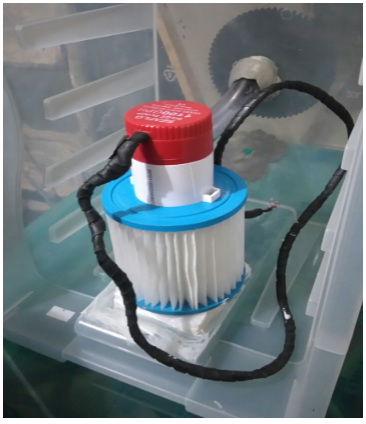
\includegraphics[width=0.5\textwidth]{figuras/bomb-real.png}
  \caption{Bomba já instalada no \textit{Clean Pool Robot}.}
  \label{fig:bomb-real}
\end{figure}
\FloatBarrier

\subsubsection{Sistema de Vedação}
O \textit{Clean Pool Robot} possui diversos equipamentos eletrônicos em seu interior que não podem ter contato com água, portanto para o sistema de vedação utilizou-se produtos que podem realizar a vedação de objetos em água. A seguir apresentamos um descritivo dos principais.

A massa Epoxi Tubolit Mep 301 foi utilizada para vedação nas saídas da caixa de processamento e da carcaça do robô, sua ação anticorrosiva e de proteção contra impactos atuou como um isolante elétrico para o CPR. Como materiais de isolação complementares, utilizou-se cola quente, fitas adesivas e o Persilox, um produto adesivo que não retrai, e depois de curado, adquire alto poder de adesão e coesão, possuindo alta performance em propriedades mecânicas, resistente a intempéries, radiação \textsf{UV} e pode ser pintado.

Foram feitos alguns protótipos para o sistema de vedação. Inicialmente, iniciou-se a construção de uma caixa usando um plástico. Nas tentativas seguintes, utilizou-se recipientes plásticos com diferentes tamanhos para a acomodação dos dispositivos eletrônicos. Esses recipientes foram adaptados com furos e vedações para atingir o objetivo. 

Nesses possíveis sistemas de vedação foram variados, além do tamanho do recipientes, os materiais que são utilizados nos locais em que poderiam ter entrada de água. No local onde é colocado a tampa, foi utilizado fitas veda rosca, o que foi suficiente para impedir a entrada de água. A maior dificuldade foi a vedação do orifício feito na tampa para a passagem dos fios, foram utilizados materiais como a cola quente e o Persilox, que apresentaram vazamento. Por fim, utilizou-se a massa Epoxi Tubolit Mep 301, que conseguiu impedir a entrada da água.

Nos testes usando a segunda versão do protótipo, CPR-02, foi abandonado o plano de internalizar a caixa de vedação com os circuitos eletrônicos. Isso porque a bolha de ar desse recipiente impedia a submersão do robô. Para a versão CPR-03, o compartimento que mantém a central de processamento foi construído de forma a permanecer flutuando na superfície da água, enquanto conectado a estrutura do robô por meio de um cabo isolado com comprimento de 2,5 metros. 

\subsection{Sistemas Lógicos}
\subsubsection{Central de Processamento}

\begin{figure}[h]
  \centering
  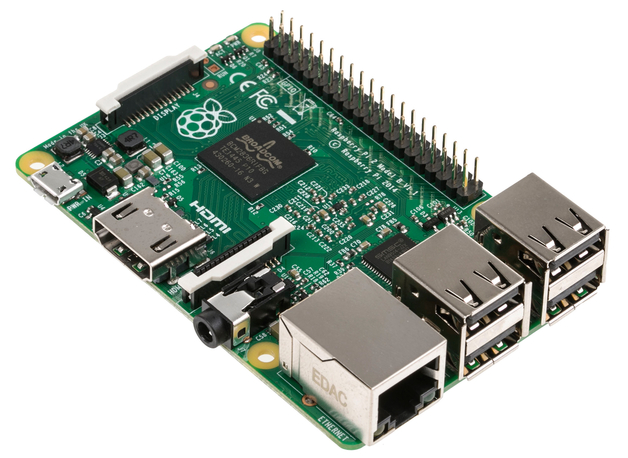
\includegraphics[width=0.5\textwidth]{figuras/rpi2b.jpg}
  \caption{\textit{Raspberry pi 2 b}.}
  \label{fig:rpi2b}
\end{figure}
\FloatBarrier

Na seleção de uma unidade de processamento, o maior fator de seleção foi conseguir uma de forma rápida e com baixo custo, além de ter uma capacidade de processamento suficiente para solucionar os primeiros requisitos vistos da integração entre a área estrutural (sensores necessários para funcionamento e acionamento de motores e bombas) e a área de \textit{software} (capacidade de programar em várias linguagens de programação e uso de APIs), e ter acesso a GPIO. Considerando esses fatos, utilizou-se uma \textit{Raspberry Pi}, suas principais características podem ser vistas abaixo:

\begin{itemize}
\item CPU de quatro núcleos ARM Cortex-A7 com frequência de processamento de 900 MHz;
\item 1GB de memória RAM;
\item 40 pinos GPIO (\textit{General Purpouse Input/Output});
\item Porta Ethernet;
\item Slot para Micro cartão SD;
\end{itemize}

Porém, por sua limitação de pinos GPIO e a necessidade de muitos pinos para analisar sinais analógicos, utilizou-se também Arduino, que vem com conversor A/D. Isso proporcionou a continuidade do trabalho de implementação que já vinha sendo feito sem muitas mudanças devido a alterações trazidas pela área eletrônica.

\begin{figure}[h]
  \centering
  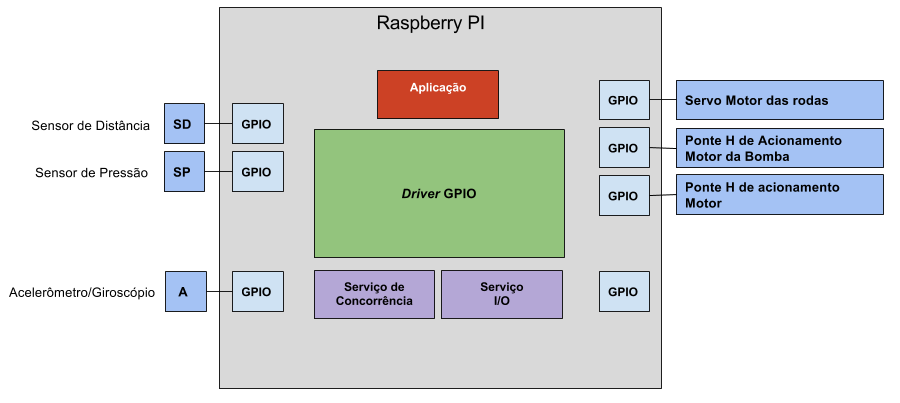
\includegraphics[width=\textwidth]{figuras/schema-eletro-soft.png}
  \caption{Esquemático eletrônica/\textit{software}.}
  \label{fig:schema-eletro-soft}
\end{figure}
\FloatBarrier

A Figura \ref{fig:schema-eletro-soft} apresenta um esquemático da relação entre as áreas de eletrônica e \textit{software}, por meio da \textit{raspberry pi}. Os periféricos fornecem os dados que, por sua vez, serão passados ao driver por meio de dispositivo de \textit{hardware} (GPIO).  O \textit{driver} é responsável por permitir a comunicação entre o \textit{hardware} e o \textit{software} que, na figura, é representado pelos serviços que deve fornecer ao sistema. Cada serviço trata os dados de entrada conforme a especificidade solicitada e, em seguida, retorna uma saída para um atuador, por meio do \textit{driver}.

A \textit{raspberry pi} recebe o código fonte que controla o robô. Esse código segue a estrutura definida pela arquitetura na Figura \ref{fig:schema-arch}:

\begin{figure}[h]
  \centering
  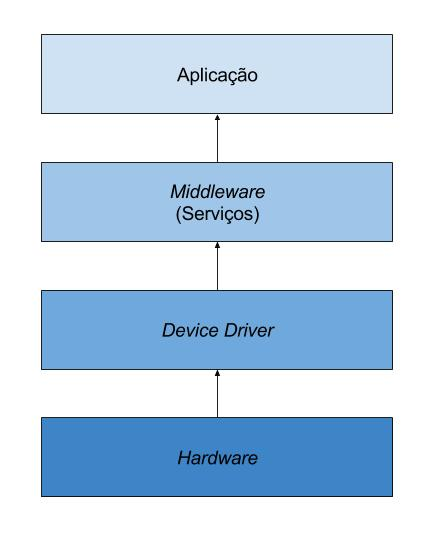
\includegraphics[width=0.4\textwidth]{figuras/schema-arch.jpg}
  \caption{Arquitetura de \textit{software}.}
  \label{fig:schema-arch}
\end{figure}
\FloatBarrier

O sistema segue uma arquitetura em camadas. A partir do \textit{hardware} os dados serão capturados. O \textit{driver} fará a ponte de comunicação entre o \textit{hardware} e o \textit{middleware}, permitindo que os dados possam ser trabalhados pela aplicação de negócio. A aplicação de negócio utilizará os serviços disponíveis pelo \textit{middleware}, afim de tratar os dados recebidos e fornecer instruções ao robô.

\textit{Middleware} é um \textit{software} que conecta outros componentes de \textit{software}. Uma camada de infraestrutura que viabiliza o desenvolvimento de aplicações voltadas ao negócio. Provê serviços que serão amplamente utilizados pela aplicação de negócio \cite{oracle2016}. O \textit{middleware} fornecerá serviços base para o robô, como ativação dos motores, escova e uso dos sensores.

A Figura \ref{fig:layers-soft} detalha melhor a comunicação entre as camadas propostas da arquitetura, considerando-se os serviços a serem utilizados e as funcionalidades na camada da aplicação.

\begin{figure}[h]
  \centering
  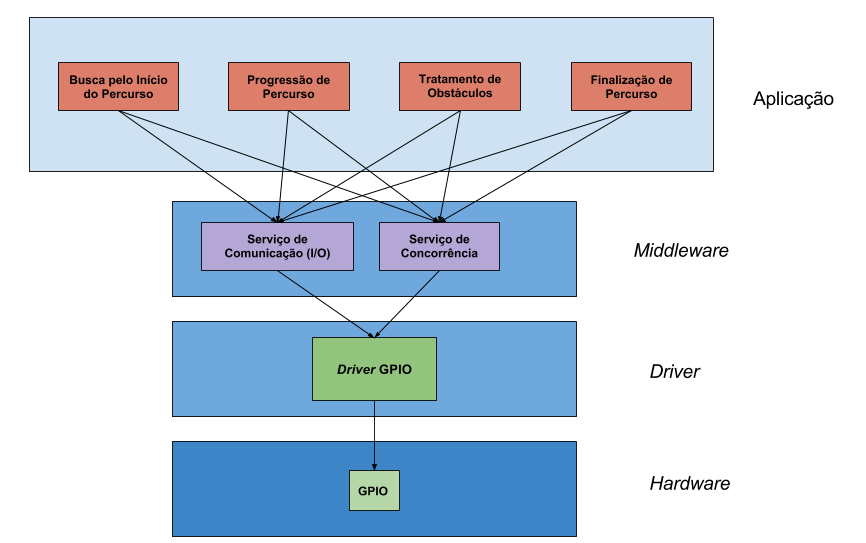
\includegraphics[width=\textwidth]{figuras/layers-soft.png}
  \caption{Visão estendida das camadas da arquitetura do \textit{software}.}
  \label{fig:layers-soft}
\end{figure}
\FloatBarrier

A camada de serviço é a camada que faz a integração entre os componentes de \textit{hardware} e os de software. Há dois serviços disponíveis no CPR: o serviço de comunicação (I/O) e o serviço de concorrência.

Esse serviço tem por propósito fazer a ponte de comunicação entre o driver e a aplicação. Dessa forma, a camada de serviço, por meio do serviço de I/O, deixa invisível para a camada de aplicação como se dá o processo de comunicação com as camadas mais baixas. Isso permite melhor entendimento do código, bem como a possibilidade de refatoração mais simples, na medida em que há um desacoplamento entre as duas partes, comunicação e aplicação. Assim, uma alteração na camada de serviço não terá impacto na camada superior, de serviço, pois a interface entre as duas se manterá. As mudanças internas à camada não interferem no funcionamento de outra.

\begin{lstlisting}[language=Python, label=services, caption=Camada de Serviço]
#!/usr/bin/env python -u
import pinout as pin
import time
import serial
import RPi.GPIO as GPIO
import time 
#Configura a serial e a velocidade de transmissao
pwm=GPIO.PWM(pin.SERVO_WHEELS,50)
pwm.start(5)

pwm_dute = GPIO.PWM(pin.SERVO_PUMP,50)
pwm_dute.start(5) 

def start_arduino():
    arduino_communication = serial.Serial("/dev/ttyAMA0", 115200)
    return arduino_communication

def read_arduino(arduino_communication):
    #print "esperando resposta"
    response = arduino_communication.read()
    print response
    return response     

def write_arduino(arduino_communication, line):
    arduino_communication.write(line)
    return

def activate_pump(arduino_communication):
   write_arduino(arduino_communication, 'G')
   time.sleep(0.1)
   #read_arduino(arduino_communication) 
   return True

def deactive_pump(arduino_communication):
    write_arduino(arduino_communication, 'H')
    time.sleep(3)
    #read_arduino(arduino_communication)
    return False

def activate_brush():
    GPIO.output(pin.BRUSH, GPIO.HIGH)
    return True

def deactive_brush():
    GPIO.output(pin.BRUSH, GPIO.LOW)
    return False

def turn_servos_wheels(angle):
    duty = float(angle)/20 + 2.5
    pwm.ChangeDutyCycle(duty)
    time.sleep(0.8)      
    return

def turn_servo_pump(angle, direction):
    if (direction == 1):
      if angle == 0:
        teste = 0
      elif (angle == 90):
        pwm_dute.ChangeDutyCycle(50)
        time.sleep(1.71)
      elif angle == 180:
        pwm_dute.ChangeDutyCycle(50)
        time.sleep(0.74)
      elif angle == 270:
        pwm_dute.ChangeDutyCycle(50)
        time.sleep(1.1)
      else:
        pwm_dute.ChangeDutyCycle(50)
        time.sleep(6.5)
    else:
      if angle == 0:
        pwm_dute.ChangeDutyCycle(2.5)
        time.sleep(0)
      elif angle == 90:
        pwm_dute.ChangeDutyCycle(2.5)
        time.sleep(0.24)
      elif angle == 180:
        pwm_dute.ChangeDutyCycle(2.5)
        time.sleep(0.54)
      elif angle == 270:
        pwm_dute.ChangeDutyCycle(2.5)
        time.sleep(0.905)
      else:
        pwm_dute.ChangeDutyCycle(2.5)
        time.sleep(1.2)
   
    pwm_dute.ChangeDutyCycle(100) 
    return
\end{lstlisting}

O serviço de concorrência tem por objetivo abstrair da aplicação questões relacionadas a tarefas que fazem uso do processamento ou de um canal ao mesmo tempo. Isso será comum nas tarefas relativas aos sensores, que devem estar aptos a exercerem suas funções o máximo de tempo possível. Assim, o serviço de concorrência fica responsável por permitir que eles atuem nesses termos, sem que um interfira nas atividades do outro.

\begin{lstlisting}[language=Python, label=threads, caption=Camada de Concorrência]
#!/usr/bin/env python -u
import thread
import communication as com
import time
semaphore = thread.allocate_lock()
def request_distance(queue, arduino_communication, request_type):
  while True:
    semaphore.acquire()
    distance = 0
    com.write_arduino(arduino_communication,request_type)
    time.sleep(0.1)
    distance = com.read_arduino(arduino_communication)
    queue.put(distance)
    time.sleep(0.1)
    semaphore.release()
  return distance

def request_pressure(queue, arduino_communication, request_type):
  while True:
    semaphore.acquire()
    #print "Requisitando pressao - " + request_type
    com.write_arduino(arduino_communication,request_type)
    time.sleep(0.05)
    pressure = com.read_arduino(arduino_communication)
    queue.put(pressure)
    semaphore.release()
  return
\end{lstlisting}

\begin{figure}[h]
  \centering
  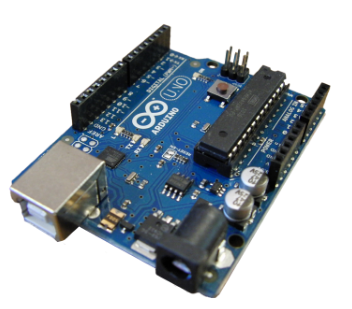
\includegraphics[width=0.5\textwidth]{figuras/arduino.png}
  \caption{Arduino Uno.}
  \label{fig:arduino}
\end{figure}
\FloatBarrier

O Arduino Uno foi escolhido, a princípio, para facilitar o tratamento do sensor de pressão MPX-4250, que possui saída analógica. Trabalhar com   conversão A/D na \textit{Raspberry pi} requer o uso demasiado de pinos (no mínimo 9 pinos para controlar dois sensores, utilizando-se de multiplexadores).  Uma vez que o Arduino Uno foi incluído no sistema, delegou-se  a ele também o trabalho de controlar os sensores de distância HC-SR04, visto  que  estes são módulos desenvolvidos para funcionar no Arduino. Porém, por não funcionar de forma ideal na água, os sensores de distância ultrassônicos foram substituídos por  sensores infravermelho E18-D0NK. Ele retorna um nível lógico baixo quando encontra um obstáculo.

Mesmo com o sensor de pressão funcionado e com todas suas implementações prontas, para limitar o número de variáveis a serem analisadas nos testes do protótipo desenvolvido neste relatório, ele não foi testado na fase final de integração. Mas, para a sua incorporação no sistema, é necessário apenas a inclusão de sua rotina dentro do programa principal, e fazer os ajustes finais dele incorporado com todo o robô.

Como alguns dos componentes de \textit{hardware} responsáveis pela coleta de dados estão vinculados ao Arduino, foi necessário o desenvolvimento de protocolo de comunicação entre a Raspberry pi e o Arduino. A Código abaixo apresenta o código desenvolvido para o Arduino, com o intuito de receber solicitações da raspberry pi e retornar com a informação requerida.

\begin{lstlisting}[language=C++, label=arduino-code, caption=Código Arduino]
#define REAR_DISTANCE_SENSOR 4
#define LEFT_DISTANCE_SENSOR 7
#define RIGHT_DISTANCE_SENSOR 12
#define FRONT_DISTANCE_SENSOR 13
#define INTERNAL_PRESSURE A1
#define EXTERNAL_PRESSURE A5
#define PUMP 8
#define BRUSH_FRONT 9
#define BRUSH_BACK 10

#define REQUEST_INTERNAL_PRESSURE 'A'
#define REQUEST_EXTERNAL_PRESSURE 'B'
#define REQUEST_FRONT_DISTANCE 'C'
#define REQUEST_REAR_DISTANCE 'D'
#define REQUEST_LEFT_DISTANCE 'E'
#define REQUEST_RIGHT_DISTANCE 'F'
#define MOTOR_PUMP_ON 'G'
#define MOTOR_PUMP_OFF 'H'
#define BRUSH_FRONT_ON 'I'
#define BRUSH_FRONT_OFF 'J'
#define BRUSH_BACK_ON 'K'
#define BRUSH_BACK_OFF 'L'

int output = 3;
int value;
byte data_rpi;
char data_request;

void setup()
{
  Serial.begin(115200);
  pinMode(3, OUTPUT);
  pinMode(REAR_DISTANCE_SENSOR,INPUT);  
}

void send_pressure(int pin)
{
  float pressure = readPressure(pin);
  float pressure_result;
  
  if (pin == A1)
  {
    pressure_result = pressure;
  } else
  {
    pressure_result = pressure + 20000;  
  }

  delay(500);
  Serial.println(pressure_result);
} 

float readPressure(int pin)
{
    int pressureValue = analogRead(pin);
    float pressure=((pressureValue/1024.0)+0.04)/0.0000369; //convertendo para pascal
    
    return pressure;
}


void send_distance (int pin)
{
  pinMode(pin,INPUT);
  int state = digitalRead(pin);
  
  if (state == HIGH)
  {
    Serial.println('N');
  } else
  {
    Serial.println('S');
  } 
}

void write_uart( byte data )
{
  Serial.println(data);
}

void turn_on_engine(int pin)
{
   pinMode(pin,OUTPUT);
   digitalWrite(pin,LOW);
   Serial.println("Ligando bomba");
}

void turn_off_engine(int pin)
{
   pinMode(pin,OUTPUT);
   digitalWrite(pin,HIGH);
   Serial.println("Desligando bomba");
}

void loop()
{
  if(Serial.available())
  {
    data_request = Serial.read();

    switch(data_request)
    {
      case REQUEST_INTERNAL_PRESSURE:
        send_pressure(INTERNAL_PRESSURE);
      break;

      case REQUEST_EXTERNAL_PRESSURE:
        send_pressure(EXTERNAL_PRESSURE);
      break;

      case REQUEST_FRONT_DISTANCE:
        send_distance(FRONT_DISTANCE_SENSOR);   
      break;
    
      case REQUEST_REAR_DISTANCE:
        send_distance(REAR_DISTANCE_SENSOR);   
      break;
      
      case REQUEST_LEFT_DISTANCE:
        send_distance(LEFT_DISTANCE_SENSOR);   
      break;
    
      case REQUEST_RIGHT_DISTANCE:
        send_distance(RIGHT_DISTANCE_SENSOR);   
      break;
  
      case MOTOR_PUMP_ON:
        turn_on_engine(PUMP);
      break;

      case MOTOR_PUMP_OFF:
        turn_off_engine(PUMP);
      break;
    
      case BRUSH_FRONT_ON:
        turn_on_engine(BRUSH_FRONT);
      break;
      
      case BRUSH_FRONT_OFF:
        turn_off_engine(BRUSH_FRONT);
      break;
    
      case BRUSH_BACK_ON:
        turn_on_engine(BRUSH_BACK);
      break;
    
      case BRUSH_BACK_OFF:
        turn_off_engine(BRUSH_BACK);
      break;
    }
  }
}
\end{lstlisting}

\subsubsection{Controle de Tensão}
Tanto a \textit{Raspberry pi} e o Arduino precisam ser alimentados com 5 volts e ter uma corrente limitada para não queimarem. Dessa forma, foi decidido usar reguladores de tensão L7805. Estes circuitos integrados são fáceis de serem adquiridos, além de baratos, e eles reduzem uma tensão de até 35Vcc. Portanto, para uma alimentação de 12Vcc esse CI funciona de forma adequada, além disso, ele disponibiliza uma corrente de saída igual a requerida pelo sistema, com um limite máximo de 1,5A.
Para evitar ruídos na alimentação de tensão foram usados dois capacitores de acoplamento, como indicado no datasheet do regulador de tensão.

Para ter corrente suficiente para todo sistema foram construídos 3 módulos com o CI do regulador de tensão e os capacitores de acoplamento: um módulo seria para alimentar a \textit{Raspberry pi}, e os sinais enviados pela GPIO da mesma; outro módulo seria para alimentar o Arduino e os sinais enviados pela GPIO do mesmo; e um último módulo para fazer a alimentação dos sensores e modulo dos relés, para garantir que nenhum sensor ou módulo fique sem alimentação, ou que alguma parte do circuito puxe mais que 1,5A.

\begin{figure}[h]
  \centering
  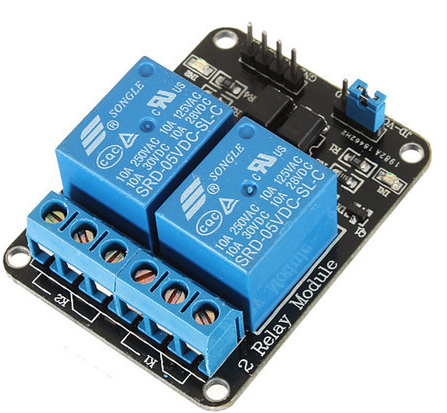
\includegraphics[width=0.4\textwidth]{figuras/rele.png}
  \caption{Rele de quatro módulos modelo SRD-05VDC-SL-C.}
  \label{fig:rele}
\end{figure}
\FloatBarrier

Para acionar os sistemas de alta tensão (motores e bomba) com circuitos de baixa tensão (\textit{Raspberry pi}) foram utilizados relés.  Com baixas tensões, ele induz um campo eletromagnético sobre uma bobina, o que faz com que o relé deixe passar a tensão que está na entrada comum para a saída do estado de circuito fechado. Caso não haja essa alimentação, o relé mantém-se em aberto, efetivamente funcionando como um interruptor.  Como é desejado que em um dos estados o circuito acione o motor e no outro o motor não funcione, foi projetado o circuito eletrônico para só acionar o motor em fechado. No estado aberto o motor está em circuito aberto, não sendo acionado. O modelo escolhido é acionado com tensão de 5Vcc, e os relés aguentam tensões de 250Vca ou 30Vcc, com corrente máxima de 10A.

\subsubsection{Sistema de Sensoriamento}
São utilizados sensores de distância com o intuito de permitir ao robô a identificação do espaço entre ele e qualquer objeto à sua frente. Dessa forma, torna-se possível o percurso predeterminado do robô. Isso é importante para evitar colisões com as paredes da piscina e obstáculos a alturas que o sensor possa detectar. Inicialmente foi escolhido um sensor de distância ultrassônico, modelo HCSR04.

Entretanto, por causa da vedação, a onda sonora perdia uma grande quantidade de energia e não detectava as distâncias de baixo d’água de forma adequada, por isso o sensor de distância foi alterado para um sensor infravermelho E18-D0NK. Este módulo trabalha com um alcance ajustável entre 3 cm e 80 cm e transmite um sinal digital HIGH (sem obstáculo) ou LOW (com obstáculo) para o arduíno, dependendo da proximidade do sensor com qualquer objeto opaco a sua frente e a distância regulada para o sensor. É portanto um sistema simples, porém robusto. O sistema de distância com foto-transistor é ideal para o projeto por permitir isolamento com uma camada de plástico transparente sem que haja interferência na detecção de qualquer obstáculo. Testes foram feitos com o sensor submerso cerca de 10 cm e ele foi capaz de detectar a parede a uma distância mínima de 9 cm quando em baixo d'água.

O sensor de pressão proposto funciona com o princípio de materiais piezoelétricos, um líquido entra dentro da câmara e proporciona uma pressão nas paredes da câmara. Esta pressão gera uma diferença de potencial no material. Com essa diferença de potencial é possível, usando um conversor AD (Analógico/Digital), saber a pressão dentro da câmara. Esse sensor sera utilizado para medir a pressão dentro da câmara onde se encontra a bomba de sucção, permitindo que a bomba só trabalhe dentro da pressão ideal de funcionamento. Caso algo entupa a entrada da sucção esse sensor detectará uma queda na pressão interna e, por \textit{software}, o problema será tratado.

Como citado anteriormente esse módulo foi testado independente do conjunto total mostrando funcionamento, porem não foi incorporado nos testes finais do protótipo, por questões de limitação de variáveis para localização de erros.

\subsubsection{Sistema de Rotação do Robô}
Foi definido pelo projeto que a propulsão do robô será gerada pela bomba de filtragem. O direcionamento consiste em dispor de um único cano capaz de rotacionar em 360 graus para se posicionar na direção desejada conforme o robô segue seu percurso.

Conforme o robô segue seu caminho, as rodas devem ser capazes de se manter em duas posições: horizontal e vertical. Para tanto, um sistema de servos com rotação de 180 graus foi escolhido, similar ao esquema de propulsão.

Servos motores são utilizados para rotacionar um eixo até uma posição desejada. Esses motores são normalmente motores de alto torque. Dois servos (Micro Servo 9g SG90 TowerPro) serão utilizados para rotacionar as rodas, o principal motivo de escolher esse modelo é ele ter torque suficiente para mover as mesmas e ter baixo custo, E para mover a saída de água da bomba foi escolhido um servo motor (SM-S4306R) com maior liberdade de rotação (360 graus) e uma maior torque.

\begin{figure}[h]
  \centering
	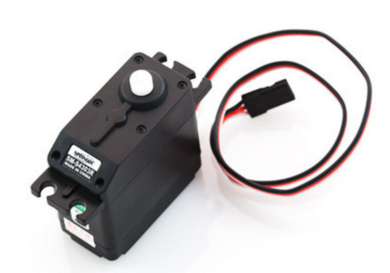
\includegraphics[height=5cm]{figuras/servant-motor.png}
	\quad
	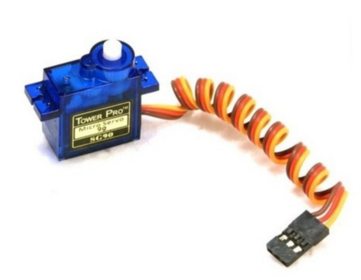
\includegraphics[height=5cm]{figuras/micro-motor.png}
  \caption{Servo-motor e motor}
  \label{fig:plastic-wheel-base}
\end{figure}
\FloatBarrier

Abaixo estão descrito as principais características dos servos escolhidos:


\begin{table}[h]
\centering
\caption{Servos e suas Características}
\label{char-servo}
\begin{tabular}{@{}cll@{}}
\toprule
\textbf{Servos}                   & SM-S4306R                          & Micro Servo 9g SG90 TowerPro       \\ \midrule
Tensão de Operação (V)            & 4,8V - 6,0V                        & 3,0V - 7,2V                        \\
Velocidade                        & 60RPM (4.8V) - 50RPM (6.0V)        & 0.12 seg/60 graus (4,8V) sem carga \\
\multicolumn{1}{l}{Torque Máximo} & 5,0 Kg*cm (4.8V) e 6.2 kg*cm(6.0V) & 1,2 Kg*cm (4.8V) e 1.6 kg*cm(6.0V) \\ \bottomrule
\end{tabular}
\end{table}

Foram feitos testes com os servos motores de modo que se pudesse validar o seu acionamento via software(através de rotinas já definidas na camada de serviço). Para o modelo Micro Servo 9g SG90, a validação de seu funcionamento prosseguiu sem muitos problemas o grau do seu giro era facilmente controlado via software. Entretanto, com o modelo SM-S4306R a equipe obteve bastante problemas nos ajustes de seu giro, de modo que foram necessárias a realização de ajustes finos via \textit{software} para que seu giro fosse mais próximo do desejado.

\subsubsection{Circuito}
Para a alimentação da \textit{raspberry Pi 2} e do Arduino Uno, bem como todos os componentes alimentados em 5V (servo motores, sensores de distância, sensores de pressão e etc), a partir dos 12V oferecidos pela fonte, utilizaram-se reguladores de tensão L7805.

Conectados a \textit{raspberry Pi 2} estão os servo motores SG90 e e S4306, pelos pinos 16 e 11 respectivamente. Para o controle dos motores dos rolos de limpeza e da bomba, utilizaram-se relés para fazer o chaveamento com a tensão de 12V da fonte.

A \textit{raspberry Pi 2} e o Arduino Uno são conectados por porta serial TX e RX e se comunicam via UART (\textit{Universal Asynchronous Receiver/Transmitter}). Um divisor de tensão é usado para conectar o pino TX0 de 5V do Arduino ao pino RXD de 3.3V da Raspberry Pi 2.

No Arduino estão conectados os quatro sensores de distância SR04, em portas digitais, e os dois sensores de pressão MPX4250 nas portas analógicas A0 e A1.

A figura abaixo mostra o diagrama do circuito proposto:

\begin{figure}[h]
  \centering
  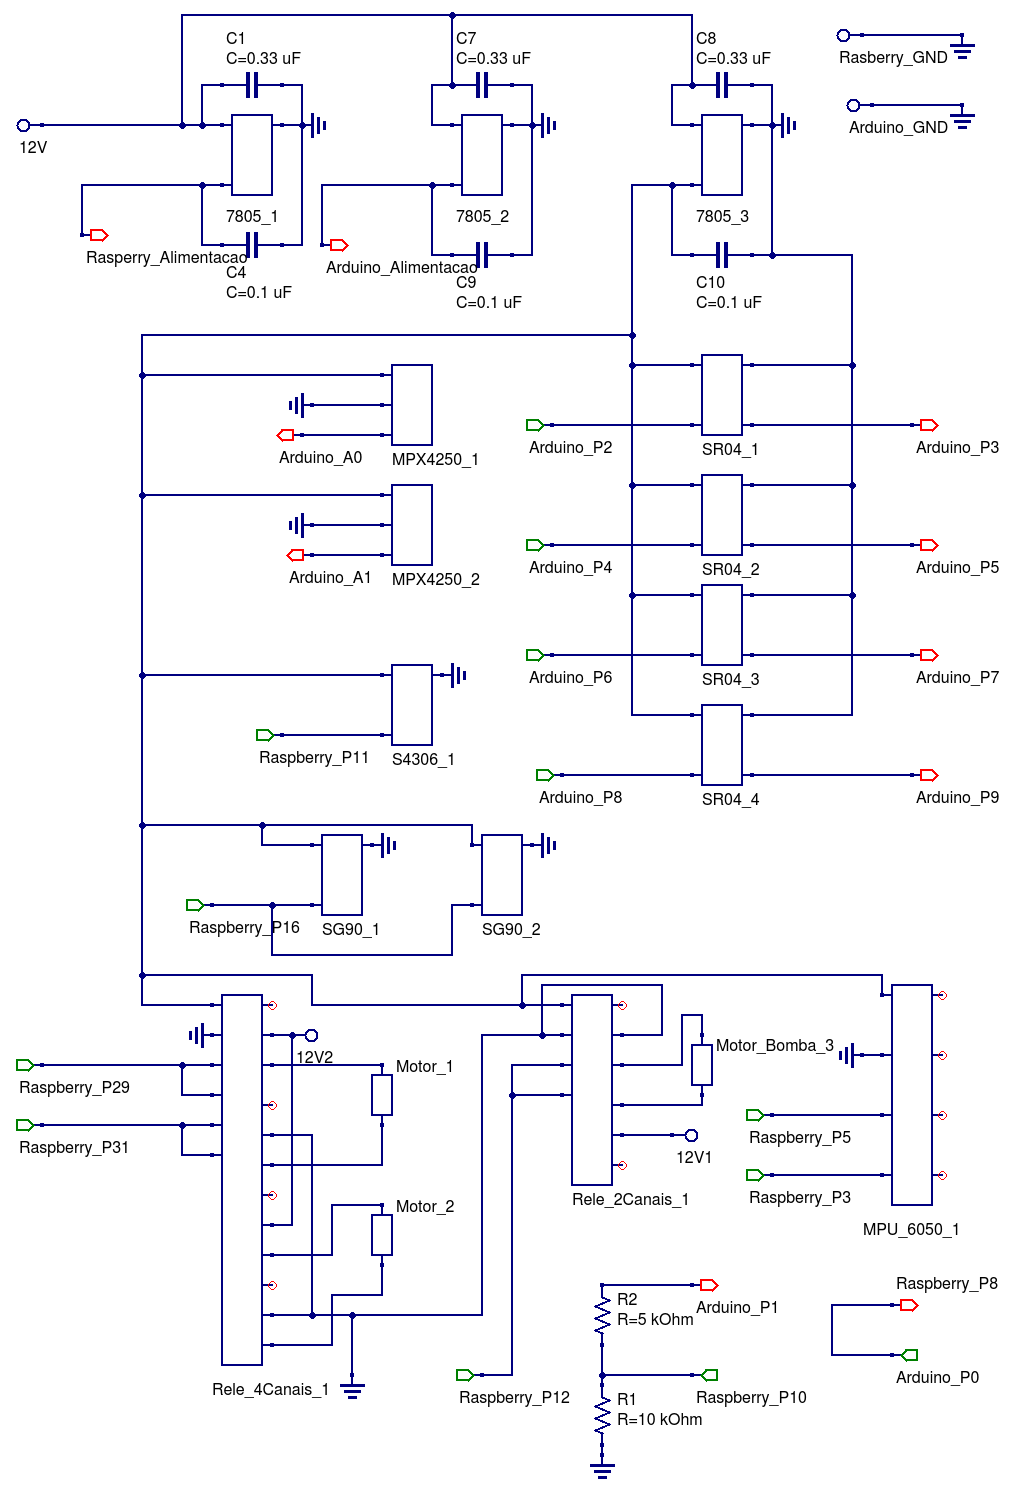
\includegraphics[width=\textwidth]{figuras/circuit.png}
  \caption{Diagrama do Circuito de Controle.}
  \label{fig:circuit}
\end{figure}
\FloatBarrier

Para ter uma maior organização foi pensando em ter um circuito impresso porém, com a necessidade de iniciar os testes e não estar decidido o sensor de distância, foi proposto fazer um circuito usando uma placa universal, onde seria possível incluir as conexões e soldas quando fosse decidido como seria detectado a distância.

Como pode ser visto na Figura \ref{fig:circuit}, a placa tem os reguladores de tensão citados anteriormente; um divisor de tensão usando três resistências, onde ele reduz a tensão de 5V do Arduino para 3.3V para que a raspberry possa ler a comunicação sem ser sobrecarregada; vários pinos para conectar e desconectar fácil a \textit{raspberry pi} e o Arduino do circuito, e conectar eles com sensores; e os fios que saem da caixa de circuito para a os sensores dentro do robô.

Foram realizados vários testes testando cada modulo da placa, para verificar o bom funcionamento de cada modulo separado, começando pelos reguladores de tensão que são a parte mais critica do circuito, já que uma falha neles causaria uma falha em todo o circuito. Nenhum módulo teve problemas nos testes, apesar que um pino quebrou e foi necessário refazer ele, mas após o conserto ter sido feito o pino funcionou como antes do teste.

\begin{figure}[h]
  \centering
  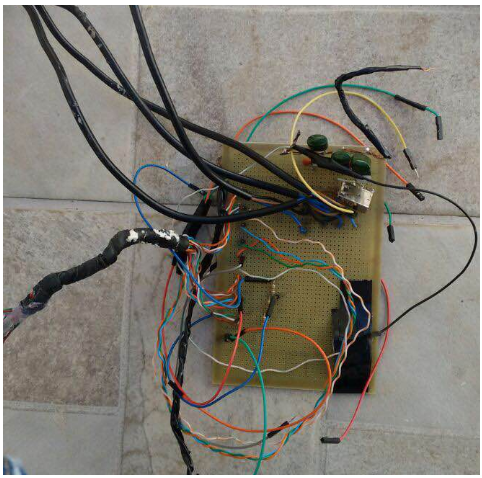
\includegraphics[width=0.5\textwidth]{figuras/circuit-real.png}
  \caption{Circuito de Controle.}
  \label{fig:circuit-real}
\end{figure}
\FloatBarrier